%% LyX 1.1 created this file.  For more info, see http://www.lyx.org/.
%% Do not edit unless you really know what you are doing.
\documentclass[12pt,english]{article}
\usepackage[T1]{fontenc}
\usepackage[latin1]{inputenc}
\usepackage{babel}
\usepackage{color}
\usepackage{graphics}
\usepackage{varioref}

\makeatletter

%%%%%%%%%%%%%%%%%%%%%%%%%%%%%% LyX specific LaTeX commands.
\providecommand{\LyX}{L\kern-.1667em\lower.25em\hbox{Y}\kern-.125emX\@}

%%%%%%%%%%%%%%%%%%%%%%%%%%%%%% User specified LaTeX commands.
%%%%%
%%%%%
%%%%%
%% Welcome!
%% if you have any question about this
%% document, please get in touch with
%% Daniel Lemire at lemire@ondelette.com
%%
%% Of course, this file was generated
%% with LyX which means that the syntax
%% might be weird at times, but I've found
%% that LyX did an excellent job overall at
%% generating clean LaTeX syntax.
%% Why do I choose LyX? Because LyX
%% doesn't come with its own LaTeX engine.
%% LyX simply use whatever tex I have.
%% There is no "proprietary gizmos" going
%% on. Also, instead of waiting for support
%% from some folk in California, I can find
%% most of the answers I need on the web,
%% for free! Oh! And LyX is free too! 
%% Good old Open Source software!
%%
%% (Sorry for the propaganda!)
%% 
%% Thanks!
%% Enjoy!
%%
%% Sept. 8th 2001
%% Grand-Pr�, NS
%%
%%%%%%%%%%
%
% Notice that this document requires quite
% a bit of macros... 
% Sorry about that!
%%%%%%%%%%%%%%
%%
\usepackage{epsfig}
\usepackage{amsmath,amssymb}
\usepackage{pslatex}
\usepackage{color}
 
 \definecolor{veryblackblue}{rgb}{0.0,0.0,0.1}
 \usepackage[pdftex,urlcolor=webblackblue,colorlinks=true]{hyperref}
 \pdfinfo{
            /Title      (Introductory Calculus- Assignment 1 Solutions)
            /Author     (Daniel Lemire, Ph.D.)
            /Subject    (This is a set of solutions for sections 1.5, 1.6, 2.1, 2.2 and 2.3 in Stewart: calculus.)
            /Keywords   (exponentials, tangents, Stewart, Solutions, limits, Acadia)
          }


\topmargin  = 0pt
\headheight = 0pt
\headsep    = 0pt

\voffset    = 0in
\hoffset    = 0in
\textheight = 230mm
\textwidth  = 164mm

\evensidemargin = 0pt
\oddsidemargin  = 0pt

\pagestyle{empty}
\usepackage{float}

%% Background of blue palette
 \definecolor{webblackblue}{rgb}{0.0,0.0,0.2}
 \definecolor{webblue}{rgb}{0.0, 0.0, 0.6}

%% Background of red palette
 \definecolor{webblackred}{rgb}{0.2,0.0,0.0}
 \definecolor{webred}{rgb}{0.6,0.0,0.0}

%% Background of green palette
 \definecolor{webblackgreen}{rgb}{0.0,0.2,0.0}                                   
 \definecolor{webgreen}{rgb}{0.0,0.6,0.0} 

%% Background of magenta palette
 \definecolor{webblackmagenta}{rgb}{0.14,0.0,0.14}                                   
 \definecolor{webmagenta}{rgb}{0.42,0.0,0.42} 

%% Background of cyan palette
 \definecolor{webblackcyan}{rgb}{0.0,0.14,0.14}                                   
 \definecolor{webcyan}{rgb}{0.0,0.42,0.42} 

%% Background of yellow pallete
 \definecolor{webblackyellow}{rgb}{0.14,0.14,0.0}                                   
 \definecolor{webyellow}{rgb}{0.85,0.85,0.0} 

 \definecolor{webdarkgray}{rgb}{0.2,0.2,0.2}

 \definecolor{webgray}{rgb}{0.75,0.75,0.75}
 \definecolor{weborange}{rgb}{1.0, 0.6, 0.0}

\renewcommand\labelenumi{\textcolor{webdarkgray}{\arabic{enumi}.}}
\newcommand{\setenumi}[1]{#1.\setcounter{enumi}{#1}}
\usepackage{dsfont}


%%
%% You might need this next line... I don't for
%% some reason... defined somewhere?
%%
%% \newcommand{\setenumi}[1]{#1.\setcounter{enumi}{#1}}
%%
%% Document should begin NOW!
%%%%%%%%%%%%%%%%%%%%%%%
%%%%%%%%%%%%%%%%%%%%%%%

\makeatother
\begin{document}

\title{Acadia University \\
\href{http://ace.acadiau.ca/math/}{Department of Mathematics and Statistics}\\
 \vspace*{3mm} \textbf{INTRODUCTORY CALCULUS 1}\\
 (MATH 1013) \\
 \vspace*{3mm} ASSIGNMENT 1 Solutions}


\author{\href{http://ondelette.com/acadia/}{Daniel Lemire}, Ph.D.}

\maketitle
\tableofcontents{}


\section{\texorpdfstring{\textcolor{webblackblue}{Functions and Models}}{Functions
and Models}}

\setcounter{subsection}{4}


\subsection{\noindent \texorpdfstring{\textcolor{webblue}{Exponential Functions}}{Exponential Functions}}

\begin{enumerate}
\item [\setenumi{14}] 

\begin{enumerate}
\item We say that two functions \( f \) and \( g \) are reflected about
a line \( y=a \) if \( f(x)-a \) and \( g(x)-a \) are equal but
have opposite signs for all \( x \). Therefore, in the present case,
we need to find a function \( f(x) \) such that \( f(x)-4=4-e^{x} \)
and that's \( f(x)=8-e^{x} \) (see Fig. \ref{refy4}).
\begin{figure}
[h]

{\centering 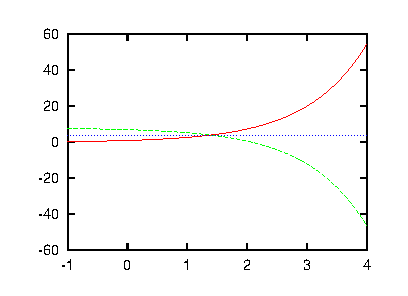
\includegraphics{question1_5_14} \par}


\caption{\label{refy4}Reflection about the line \protect\( y=4\protect \)}
\end{figure}

\item Two functions \( f \) and \( g \) are reflected about the line \( x=a \)
if \( f(a+x)=g(a-x) \) for all \( x \). The function we are looking
for is \( f(x+2)=e^{2-x} \) because \( g(x)=e^{x} \). We finally
substitute \( z=x+2 \) (or \( x=z-2 \)) to obtain \( f(z)=e^{4-z} \)
(see Fig. \ref{refy4b}).
\begin{figure}
[h]

{\centering \includegraphics{question1_5_14b} \par}


\caption{\label{refy4b}Reflection about the line \protect\( x=2\protect \)}
\end{figure}

\end{enumerate}
\item [\setenumi{16}]\label{enum:question16}Looking at the graph, we can
observe that \( f(0)=2 \) and \( f(2)=\frac{2}{9} \). Since \( f(x)=Ca^{x} \),
we have that\begin{equation}
\label{eqntrivial}
Ca^{0}=2
\end{equation}
and\begin{equation}
\label{eqnnotsotrivial}
Ca^{2}=\frac{2}{9}.
\end{equation}
From equation \ref{eqntrivial}, we see right away that \( C=2 \)
and therefore, equation \ref{eqnnotsotrivial} becomes\[
a^{2}=\frac{1}{9}\]
which implies that \( a=\pm \frac{1}{3} \). However, we must reject
the solution \( a=-\frac{1}{3} \) because the function \( f(x)=2\times \left( \frac{-1}{3}\right) ^{x} \)
implies \( f(1)=\frac{-2}{3} \) which doesn't agree with the graph.
We have one remaining solution and it is \[
f(x)=2\times \left( \frac{1}{3}\right) ^{x}.\]

\item [\setenumi{18}]We will assume that the highest paying job at the end
of the month must be chosen. The first job pays \( 1,000,000 \) over
a month. How much pays the second one? Setting up the equation is
not very difficult, we readily see that it pays%
\footnote{We chose a month with 30 days.
} \begin{equation}
\label{geom}
pay=\sum _{n=1}^{30}2^{n-1}.
\end{equation}
How much is it? The formula \ref{geom} is called a \textit{geometric
series}. We can solve it rather easily, we simply evaluate \( pay-2\times pay \)
by using formula \ref{geom} which gives\begin{eqnarray*}
pay-2\times pay= & \sum _{n=1}^{30}2^{n-1}-2\times \sum _{n=1}^{30}2^{n-1} & \\
= & \sum _{n=1}^{30}2^{n-1}-\sum _{n=2}^{31}2^{n-1} & \\
= & 2^{0}-2^{30} & 
\end{eqnarray*}
We then solve for \( pay \) in \( pay-2\times pay=1-2^{30} \) which
is very easy since \( pay-2\times pay=-pay \), and we finally have
\( pay=2^{30}-1 \). It should be noted here that \( 2^{30} \) is
a very big number (about one billion or \( 1,073,741,824 \)).
What is the lesson here? Exponential functions can increase \textbf{\textcolor{red}{very
fast}}%
\footnote{Most modern computer architectures are 32 bits (Windows, Linux and
even the new gaming consoles). Therefore, the highest integer value
most programmers will ever expect is \( 2^{32}-1 \). Of course, newer
computer architectures will probably be 64 bits and integers will
go up to \( 2^{64}-1 \). Will that be a big improvement? How much
bigger is \( 2^{64} \) with respect to \( 2^{32} \)?
}. 
\item [\setenumi{24}]

\begin{enumerate}
\item Given that the half-life is 15 hours, after 15 hours, we have \( 2/2=1 \)
g left (by definition). After another 15 hours (for a total of 30
hours), we have \( 1/2 \) g left, and after yet another 15 hours
(for a total of 30 hours), we have \( 1/4 \) g left. Finally, after
60 hours, we'll have \( 1/8 \) g left%
\footnote{It is also possible to deduce this result from equation \ref{decayofsodium}.
}.
\item Since the decay is exponential, we have that \begin{equation}
\label{expbasic}
m(x)=Ca^{x}.
\end{equation}
 First of all, \( m(0)=2 \) and therefore \( C=2 \) (see equation
\ref{eqntrivial} \vpageref{eqntrivial}). We have that after 15 hours,
the mass must be half, so \begin{equation}
\label{halflife}
m(15)=1.
\end{equation}
Combining equations \ref{expbasic} and \ref{halflife}, we get that\begin{equation}
\label{a15}
2a^{15}=1
\end{equation}
 \( 2a^{15}=1 \) and we must now solve for \( a \). One way to do
it (assuming we don't know about logarithms) is to take the equation
\ref{a15}to the power \( \frac{1}{15} \) to get \[
a=\frac{1}{2^{1/15}}\cong \frac{1}{1.047}\cong 0.9548.\]
 This means that the mass of our sample goes down according to the
equation%
\footnote{Actually, your calculator or mathematical software is likely to evaluate
this function using the formula \( e^{(1-x/15)\ln 2} \) instead.
We will come back to logarithms and their applications later in the
course. 
} \begin{equation}
\label{decayofsodium}
m(x)=2\left( \frac{1}{2}\right) ^{\frac{x}{15}}=\left( \frac{1}{2}\right) ^{\frac{x}{15}-1}.
\end{equation}

\begin{figure}
[h]

{\centering \includegraphics{question1_5_24} \par}


\caption{Mass of sodium vs time according to equation \ref{decayofsodium}}
\end{figure}

\item Amount after 4 days? What you \textcolor{red}{must not} do here is
substitute \( 4 \) in equation \ref{decayofsodium}. The correct
reasoning is to first convert 4 days in hours. We have 24 hours for
every day, so 4 days is \( 4\times 24=96 \) hours. Therefore, the
remaining mass will be\[
m(96)=\left( \frac{1}{2}\right) ^{\frac{96}{15}-1}\cong 0.02.\]

\end{enumerate}
\end{enumerate}

\subsection{\texorpdfstring{\textcolor{webblue}{Inverse Functions and Logarithms}}{Inverse Functions and Logarithms}}

\begin{enumerate}
\item [\setenumi{18}]

\begin{enumerate}
\item We have to solve the equation \[
3=3+x^{2}+\tan (\pi x/2)\]
which simplifies to \[
\tan (\pi x/2)=-x^{2}.\]
Now, some of you might think that life is pretty hard (and it sometimes
is!). But wait! What is \( \tan (0) \)? \( 0 \) of course! And what
is \( x^{2} \) evaluated at \( 0 \)? \( 0 \) of course! So we found
a solution which we will assume to be unique and we conclude that
\( f^{-1}(3)=0 \) (See Fig. \ref{equation1to1maybe}).
\item \textcolor{red}{You must not try to evaluate \( f^{-1}(5) \)!} We
write \( x_{5}=f^{-1}(5) \) and \( x_{5} \) is defined by the equation
\( f\left( x_{5}\right) =5 \). And thus \[
f\left( f^{-1}\left( 5\right) \right) =f\left( x_{5}\right) =5.\]

\begin{figure}
[h]

{\centering \includegraphics{question1_6_18} \par}


\caption{\label{equation1to1maybe}\protect\( 3+x^{2}+\tan (\pi x/2)\protect \)}
\end{figure}

\end{enumerate}
\item [\setenumi{28}]We want to compute the inverse of the following function\begin{equation}
\label{1expover1moinsx}
f(x)=\left( 1+e^{x}\right) /\left( 1-e^{x}\right) 
\end{equation}
 It is worth noting that when \( x=0 \), we get \( f(0)=2/0=\infty  \).
Since we know that \( \ln \left( e^{x}\right) =x \), we have \begin{eqnarray*}
\frac{1+e^{x}}{1-e^{x}}=y & \Longrightarrow  & \left( 1-e^{x}\right) y=1+e^{x}\\
 & \Longrightarrow  & (1+y)e^{x}=y-1\\
 & \Longrightarrow  & e^{x}=\frac{y-1}{y+1}\\
 & \Longrightarrow  & x=\ln \left( \frac{y-1}{y+1}\right) .
\end{eqnarray*}
Of course, this function isn't defined for \( \frac{y-1}{y+1}\leq 0 \)
or \( -1\leq y\leq 1 \). One could verify that \( f(x) \) in equation
\ref{1expover1moinsx} never takes these values (see also Fig. \ref{graph1exp}). 
\begin{figure}
[h]

{\centering \includegraphics{question1_6_28} \includegraphics{question1_6_28b} \par}


\caption{\label{graph1exp}\protect\( f(x)=\left( 1+e^{x}\right) /\left( 1-e^{x}\right) \protect \)}
\end{figure}
 
\item [\setenumi{36}]Recall that \( \log a^{b}=b\log a \) and \( \log _{a}a=1 \).

\begin{enumerate}
\item \( \log _{8}2=\log _{8}\left( 8^{\frac{1}{3}}\right) =\frac{1}{3}\times \log _{8}8 \)
because \( \log a^{b}=b\log a \), and since \( \log _{a}a=1 \),
\[
\frac{1}{3}\times \log _{8}8=\frac{1}{3}\]
 so that \( \log _{8}2=\frac{1}{3} \).
\item \( \ln e^{\sqrt{2}}=\sqrt{2}\ln e \) because \( \ln a^{b}=b\ln a \),
and since \( \ln e=1 \), we have \( \ln e^{\sqrt{2}}=\sqrt[]{2} \). 
\end{enumerate}
\item [\setenumi{38}]Recall that \( a^{b+c}=a^{b}a^{c} \) and \( a^{\log _{a}b}=b \)
(see equation 7 in \cite{Steward} on page 68).

\begin{enumerate}
\item \( 2^{\log _{2}3+\log _{2}5}=2^{\log _{2}3}\times 2^{\log _{2}5}=3\times 5=15 \)
\item \( e^{3\ln 2}=e^{\ln \left( 2^{3}\right) }=2^{3}=8 \)
\end{enumerate}
\item [\setenumi{42}]The logarithm has \( \left( 0,\infty \right)  \) for
its domain (it isn't defined elsewhere, at least in this course).
Therefore, in \( \ln \left( 4-x^{2}\right)  \), we need to have \( 4-x^{2}\geq 0 \)
or\begin{equation}
\label{sqrt4}
x^{2}<4.
\end{equation}
 At this point, one must be \textcolor{red}{careful}. We may think
of taking the square root on both sides of equation \ref{sqrt4} (getting
\( x<2 \)) and indeed, it is correct to do so... as long as you realize
that if \( a^{2}=b \) then so does \( \left( -a\right) ^{2}=b \)!
That is, you have to consider negative values as well... Therefore,
we have \[
x<2\]
 \textcolor{blue}{and} \[
x>-2.\]
We conclude that the domain of \( \ln \left( 4-x^{2}\right)  \) is
\( \left( -2,2\right)  \).\\
As for the range of the function... we first have to look at the range
of \( 4-x^{2} \) over \( \left( -2,2\right)  \). Clearly, the polynomial
is at its maximum when \( x=0 \) and so its range has \( 4 \) as
an upper bound. On the other hand, it has \( 0 \) as its lower bound
and therefore the range of \( 4-x^{2} \) over \( \left( -2,2\right)  \)
is \( \left( 0,4\right]  \). Since the logarithm is a strictly increasing
function, we can conclude that the range of \( \ln \left( 4-x^{2}\right)  \)
is \( \left( \ln 0,\ln 4\right]  \) or \( \left( -\infty ,\ln 4\right]  \)
or approximately \( \left( -\infty ,1.386\right]  \) (see Fig. \ref{graphln4}).
\begin{figure}
[h]

{\centering \includegraphics{question1_6_42} \par}


\caption{\label{graphln4}\protect\( f(x)=\left( 1+e^{x}\right) /\left( 1-e^{x}\right) \protect \)}
\end{figure}
 
\item [\setenumi{52}]

\begin{enumerate}
\item Starting from \( \ln \ln x=1 \), we write \( e^{1}=e^{\ln \ln x} \)
but since \( e^{\ln w}=w \), we have \( e=\ln x \) and finally,
we write \[
e^{e}=e^{\ln x}=x\]
so that \( x=e^{e} \).
\item Starting from \( e^{ax}=Ce^{bx} \), we divide both sides of the equation
by \( e^{bx} \) (which we know to be a non-zero positive number!
why?) to get \[
e^{\left( a-b\right) x}=C.\]
 We can then simply take the logarithm of both sides of the equation
to get\[
\left( a-b\right) x=\ln C\]
and therefore \( x=\frac{\ln C}{a-b} \) because \( a\neq b \).
\end{enumerate}
\item [\setenumi{58}]

\begin{enumerate}
\item We have to solve for \( t \) in \[
Q_{0}\left( 1-e^{-t/a}\right) =Q.\]
 We begin by dividing by \( Q_{0} \) both sides of the equation and
after some algebra, we get\[
e^{-t/a}=1-\frac{Q}{Q_{0}}.\]
Taking the logarithm, we get\[
\frac{-t}{a}=\ln \left( 1-\frac{Q}{Q_{0}}\right) \]
or\[
t=-a\ln \left( 1-\frac{Q}{Q_{0}}\right) \]
or\begin{equation}
\label{timefunctionQ}
t=a\ln \frac{Q_{0}}{Q_{0}-Q}
\end{equation}
because \( \ln c/b=-\ln b/c \). It should be noted that if \( Q_{0}=Q \)
(at time \( t=0 \)), then we have the logarithm of \( 0 \) or of
\( \infty  \) which is not very good! We must therefore require that
\( Q<Q_{0} \) in which case \[
\frac{Q_{0}}{Q_{0}-Q}>1\]
 and therefore \( t>0 \) (because \( \ln \left( 1\right) =0 \)).
When \( Q=0 \), we have \( t=0 \). What does equation \ref{timefunctionQ}
mean? Well, it gives us time as a function of the charge \( Q \).
When the charge is at its minimum (\( 0 \)), then \( t=0 \) and
we know that we just started recharging... as \( Q \) increases (getting
closer to \( Q_{0} \)), we can compute the corresponding number of
seconds we waited. 
\item Setting \( Q=0.9Q_{0} \) and substituting in equation \ref{timefunctionQ},
we have \begin{eqnarray*}
t & = & a\ln \frac{Q_{0}}{Q_{0}-0.9Q_{0}}\\
 & = & a\ln \frac{Q_{0}}{0.1Q_{0}}\\
 & = & a\ln \frac{1}{0.1}\\
 & = & a\ln 10
\end{eqnarray*}
and because \( a=2 \), we have \( t=2\ln 10\cong 4.6 \) seconds.
Bonus: how long for 99\% of the charge? We substitute again to get
\( t=2\ln \frac{1}{0.01}\cong 9.2 \) seconds... how long for 99.9\%
of the charge? We have \( t=2\ln \frac{1}{0.001}\cong 13.8 \) seconds...
What is happening? The logarithm grows very slowly! We can get very,
very close to full charge without waiting all that long! 
\end{enumerate}
\end{enumerate}
\begin{thebibliography}{Stewart}
\bibitem[Stewart]{Steward}James Stewart, \textit{Calculus: Concepts and Contexts} (Second Edition),
Brooks/Cole, 2001.\end{thebibliography}

\end{document}
